\documentclass[border=10pt,tikz]{standalone}
\usepackage{amsmath}
\usepackage{amssymb}
\usepackage{tikz}
\usetikzlibrary{arrows.meta,calc,decorations.pathreplacing,patterns,shapes.geometric,positioning,shadings,decorations.pathmorphing}

\begin{document}
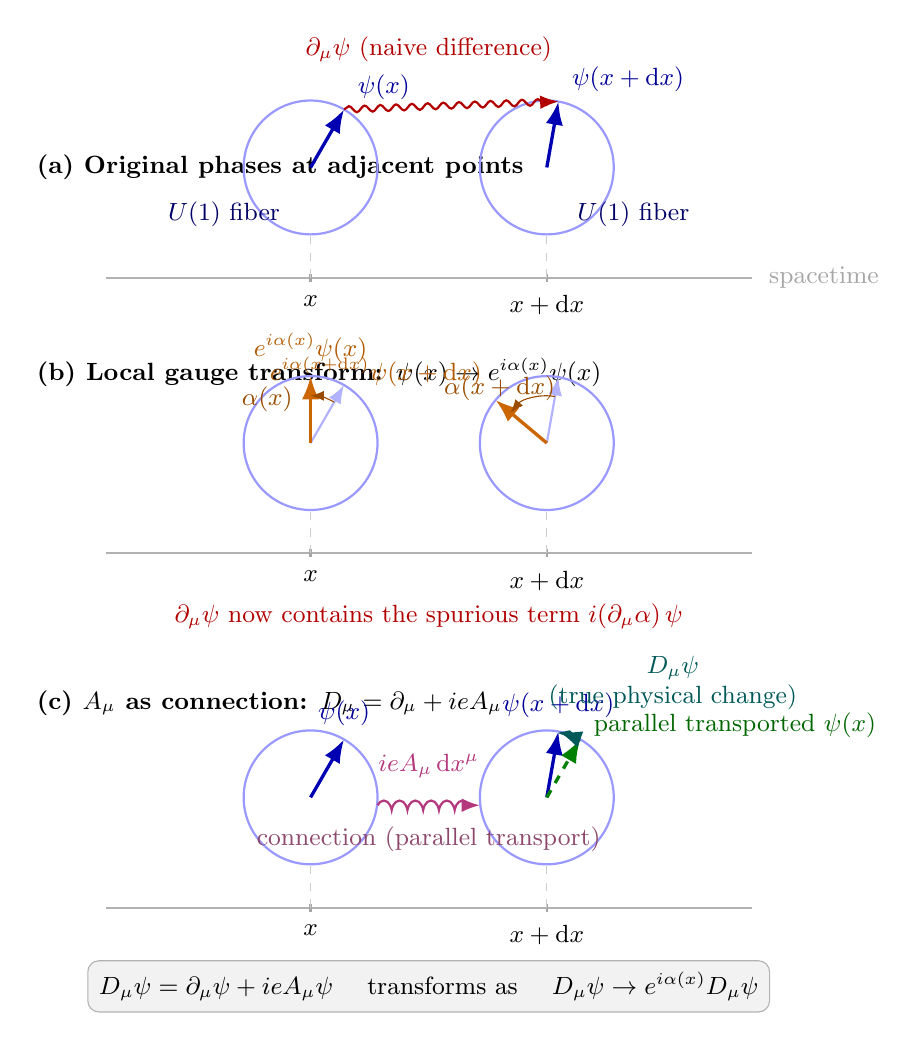
\begin{tikzpicture}[>=Latex, font=\small]

% =====================================================
% TOP ROW: original (free) phases at adjacent spacetime points x and x+dx
% =====================================================
\begin{scope}[shift={(0,3.5)}]
  \node[anchor=west] at (-3.6,0.0) {\textbf{(a) Original phases at adjacent points}};

  % Spacetime "axis" line
  \draw[gray!60, thick] (-2.6,-1.4) -- (5.6,-1.4);
  \node[gray!70, anchor=west] at (5.7,-1.4) {spacetime};

  % Point x : tick + label
  \draw[gray!70, thick] (0,-1.45) -- (0,-1.35);
  \node[anchor=north] at (0,-1.5) {$x$};

  % Point x+dx : tick + label
  \draw[gray!70, thick] (3,-1.45) -- (3,-1.35);
  \node[anchor=north] at (3,-1.5) {$x+\mathrm{d}x$};

  % U(1) fiber circles above each point
  \draw[blue!40, thick] (0,0) circle (0.85);
  \draw[blue!40, thick] (3,0) circle (0.85);

  % Fiber connecting line (vertical hint)
  \draw[gray!40, dashed, thin] (0,-1.4) -- (0,-0.85);
  \draw[gray!40, dashed, thin] (3,-1.4) -- (3,-0.85);

  % Phase arrow at x (angle theta_1)
  \draw[->, very thick, blue!70!black] (0,0) -- ({0.85*cos(60)},{0.85*sin(60)});
  \node[blue!60!black, anchor=south west] at ({0.85*cos(60)+0.05},{0.85*sin(60)}) {$\psi(x)$};

  % Phase arrow at x+dx (angle theta_2 -- slightly different)
  \draw[->, very thick, blue!70!black] (3,0) -- ({3+0.85*cos(80)},{0.85*sin(80)});
  \node[blue!60!black, anchor=south west] at ({3+0.85*cos(80)+0.05},{0.85*sin(80)}) {$\psi(x+\mathrm{d}x)$};

  % Fiber labels
  \node[blue!40!black] at (-1.1,-0.6) {$U(1)$ fiber};
  \node[blue!40!black] at (4.1,-0.6) {$U(1)$ fiber};

  % Naive comparison: partial mu psi
  \draw[->, thick, red!70!black, decorate, decoration={snake, amplitude=.4mm, segment length=2mm}]
    ({0.85*cos(60)},{0.85*sin(60)}) -- ({3+0.85*cos(80)},{0.85*sin(80)});
  \node[red!70!black] at (1.5,1.5) {$\partial_{\mu}\psi$ (naive difference)};
\end{scope}

% =====================================================
% MIDDLE ROW: after local gauge transformation
% =====================================================
\begin{scope}[shift={(0,0)}]
  \node[anchor=west] at (-3.6,0.9) {\textbf{(b) Local gauge transform: $\psi(x)\to e^{i\alpha(x)}\psi(x)$}};

  % Spacetime "axis" line
  \draw[gray!60, thick] (-2.6,-1.4) -- (5.6,-1.4);

  % Point x and x+dx ticks
  \draw[gray!70, thick] (0,-1.45) -- (0,-1.35);
  \node[anchor=north] at (0,-1.5) {$x$};
  \draw[gray!70, thick] (3,-1.45) -- (3,-1.35);
  \node[anchor=north] at (3,-1.5) {$x+\mathrm{d}x$};

  % Fiber circles
  \draw[blue!40, thick] (0,0) circle (0.85);
  \draw[blue!40, thick] (3,0) circle (0.85);
  \draw[gray!40, dashed, thin] (0,-1.4) -- (0,-0.85);
  \draw[gray!40, dashed, thin] (3,-1.4) -- (3,-0.85);

  % Original (faded) arrows
  \draw[->, thick, blue!30] (0,0) -- ({0.85*cos(60)},{0.85*sin(60)});
  \draw[->, thick, blue!30] (3,0) -- ({3+0.85*cos(80)},{0.85*sin(80)});

  % Rotated arrows (different alpha at each point)
  % at x rotate by alpha(x) ~ +30 deg
  \draw[->, very thick, orange!80!black] (0,0) -- ({0.85*cos(90)},{0.85*sin(90)});
  \node[orange!70!black, anchor=south] at ({0.85*cos(90)},{0.85*sin(90)+0.05}) {$e^{i\alpha(x)}\psi(x)$};

  % at x+dx rotate by alpha(x+dx) ~ +60 deg (different!)
  \draw[->, very thick, orange!80!black] (3,0) -- ({3+0.85*cos(140)},{0.85*sin(140)});
  \node[orange!70!black, anchor=south east] at ({3+0.85*cos(140)-0.05},{0.85*sin(140)+0.05}) {$e^{i\alpha(x+\mathrm{d}x)}\psi(x+\mathrm{d}x)$};

  % Curved arc showing alpha rotation at x
  \draw[->, thin, orange!60!black] ({0.6*cos(60)},{0.6*sin(60)}) arc (60:90:0.6);
  \node[orange!60!black] at (-0.55,0.55) {$\alpha(x)$};

  % Curved arc showing alpha rotation at x+dx
  \draw[->, thin, orange!60!black] ({3+0.6*cos(80)},{0.6*sin(80)}) arc (80:140:0.6);
  \node[orange!60!black] at (2.4,0.7) {$\alpha(x+\mathrm{d}x)$};

  % WARNING: phase difference depends on alpha(x+dx)-alpha(x)
  \node[red!70!black, align=center] at (1.5,-2.2) {$\partial_{\mu}\psi$ now contains the spurious term $i(\partial_{\mu}\alpha)\,\psi$};
\end{scope}

% =====================================================
% BOTTOM ROW: gauge field A_mu compensates -> covariant derivative
% =====================================================
\begin{scope}[shift={(0,-4.5)}]
  \node[anchor=west] at (-3.6,1.2) {\textbf{(c) $A_{\mu}$ as connection: $D_{\mu}=\partial_{\mu}+ieA_{\mu}$}};

  % Spacetime "axis" line
  \draw[gray!60, thick] (-2.6,-1.4) -- (5.6,-1.4);

  % Ticks
  \draw[gray!70, thick] (0,-1.45) -- (0,-1.35);
  \node[anchor=north] at (0,-1.5) {$x$};
  \draw[gray!70, thick] (3,-1.45) -- (3,-1.35);
  \node[anchor=north] at (3,-1.5) {$x+\mathrm{d}x$};

  % Fiber circles
  \draw[blue!40, thick] (0,0) circle (0.85);
  \draw[blue!40, thick] (3,0) circle (0.85);
  \draw[gray!40, dashed, thin] (0,-1.4) -- (0,-0.85);
  \draw[gray!40, dashed, thin] (3,-1.4) -- (3,-0.85);

  % Phase arrows
  \draw[->, very thick, blue!70!black] (0,0) -- ({0.85*cos(60)},{0.85*sin(60)});
  \node[blue!60!black, anchor=south] at ({0.85*cos(60)},{0.85*sin(60)+0.05}) {$\psi(x)$};
  \draw[->, very thick, blue!70!black] (3,0) -- ({3+0.85*cos(80)},{0.85*sin(80)});
  \node[blue!60!black, anchor=south] at ({3+0.85*cos(80)},{0.85*sin(80)+0.05}) {$\psi(x+\mathrm{d}x)$};

  % Parallel-transported phase from x to x+dx via connection A_mu
  % Show as a "ghost" arrow at x+dx that has the parallel-transported phase from x
  \draw[->, very thick, green!50!black, dashed] (3,0) -- ({3+0.85*cos(60)},{0.85*sin(60)});
  \node[green!40!black, anchor=south west] at ({3+0.85*cos(60)+0.05},{0.85*sin(60)-0.1}) {parallel transported $\psi(x)$};

  % Connection A_mu as a curving "tube" between fibers at the bottom
  \draw[->, thick, magenta!70!black, decorate, decoration={coil, aspect=0.5, segment length=2mm, amplitude=0.6mm}]
    (0.85,-0.1) -- (2.15,-0.1);
  \node[magenta!70!black] at (1.5,0.4) {$ieA_{\mu}\,\mathrm{d}x^{\mu}$};
  \node[magenta!50!black, anchor=north] at (1.5,-0.25) {connection (parallel transport)};

  % Covariant derivative result: subtracting parallel transport from psi(x+dx)
  \draw[->, very thick, teal!70!black, decorate, decoration={snake, amplitude=.4mm, segment length=2mm}]
    ({3+0.85*cos(60)},{0.85*sin(60)}) -- ({3+0.85*cos(80)},{0.85*sin(80)});
  \node[teal!70!black, align=center] at (4.6,1.45) {$D_{\mu}\psi$\\(true physical change)};

  % Equation reminder
  \node[align=center, draw=gray!60, fill=gray!10, rounded corners, inner sep=4pt] at (1.5,-2.4)
    {$D_{\mu}\psi = \partial_{\mu}\psi + ieA_{\mu}\psi$ \quad transforms as \quad $D_{\mu}\psi \to e^{i\alpha(x)} D_{\mu}\psi$};
\end{scope}

\end{tikzpicture}
\end{document}
